
\documentclass[a4paper]{article}
\usepackage[portuguese]{babel}
\usepackage[utf8]{inputenc}
\usepackage[T1]{fontenc}
\usepackage{mathtools}
\usepackage{circuitikz}
\usepackage{siunitx}
\usepackage{amsmath,amssymb}
\usepackage[a4paper, margin=1in]{geometry}
\usepackage{steinmetz}
\title{Projeto de Sistema de Controle utilizando o Método do Lugar das Raízes}

\author{
	Gabriela Gomes dos Santos \and
	Vitor Bruno de Oliveira Barth
}
\date{\today}


\begin{document}
	\maketitle
	
	% 
	% INTRODUÇÃO
	%
	\section{Introdução}
	\par Dada a Planta abaixo: 
	\par
	\vspace{2em}
	\begin{center}
	
	% 
	% CIRCUITO
	%
	\begin{circuitikz} \draw
		(0,0) node [left] {$E_{i}$} to[R=$R_1$, i_=$I_1$, o-] (3,0)
			  to[short, i_=$I_2$] (6,0)
			  to[R=$R_2$] (7.2,0)
			  to[short, -o] (11,0) node [right] {$E_{o}$}
		(3.5,0) to[short, i=$I_3$] (3.5,-2)
				to[C=$C_1$] (3.5,-4)
		        to    (9,-4)
		        to[C=$C_2$] (9,-2)  
		        to[short, , -*] (9,0)
		(6.5,-4) node[ground]{}
		;
	\end{circuitikz}
	
	% 
	% DADOS DAS RESISTÊNCIAS E CAPACITÂNCIAS
	%
	\end{center}
	\vspace{2em}
	\par E os dados:
	\vspace{1em}
	\par $R_1=$\SI{10}{\ohm}
	\par $R_2=$\SI{10}{\kilo\ohm}
	\par $C_1=$\SI{0.2}{\micro\farad}
	\par $C_2=$\SI{0.1}{\nano\farad}
	\vspace{2em}
	
	\par
	Deseja-se criar um compensador por avanço e atraso de fase para melhorar o desempenho da planta, tal que:
	\vspace{1em}
	\par $a)$ O Tempo de Assentamento ($T_s$) seja igual a \SI{0.3}{\milli\second}
	\par $b)$ O Máximo de Sobressinal ($M_p$) seja igual a \SI{20}\%
	\par $c)$ O Erro Estático de Velocidade ($K_v$) seja igual a 100$s^{-1}$
	
	% 
	% DADOS DA PLANTA
	%
	\section{Dados da Planta}\label{previous work}
	
	% 
	% FT MALHA ABERTA
	%
	\subsection{Cálculo da Função de Transferência Malha Aberta}
	\vspace{1em}

	\begin{align}
	E_o &= I_3*\frac{1}{C_2s}\\
	E_i &= I_1*[R_1+\frac{\frac{R_2C_2s+1}{C_2s} * \frac{1}{C_2s}}{\frac{R_2C_2s+1}{C_2s}+ \frac{1}{C_2s}}]
	\end{align}
	\vspace{1em}
	\par Sendo assim: 
	
	\begin{align}
	\frac{E_o}{E_i} &= \frac{I_3}{I_1}[\frac{1}{C_2s}*\frac{R_2C_1C_2s^2+C_1s+C_2s}{R_1R_2C_1C_2s^2+(R_1C_1+R_1C_2+R_2C_2)s+1}]
	\end{align}
	\vspace{0.3em}
	\par Para se encontrar o quociente $\frac{I_3}{I_1}$, utilizamos a Lei de Kirchhoff das Correntes: 
	
	\begin{align}
	I_1 &= I_2+I_3
	\end{align}
	
	\vspace{0.3em}
	\par Ao verificar que $C_1$ está em um ramo paralelo à $C_2$ e $R_2$, conclui-se que a diferença de potencial em ambos é a mesma. Logo, pode-se dizer que:
	
	\begin{align}
	I_2*\frac{1}{C_1s} &= I_3*[R_2+\frac{1}{C_2s}]	\\
	I_2 &= I_3*\frac{R_2C_1C_2s+C_1}{C_2}
	\end{align}
	
	\vspace{0.3em}
	\par Substituindo $(6)$ em $(4)$, temos:
	
	\begin{align}
	I_1 &= I_3*\frac{R_2C_1C_2s+C_1}{C_2} + I_3\\
	\frac{I_3}{I_1} &= \frac{C_2}{R_2C_1C_2s+C_1+C_2}
	\end{align}
	
	\vspace{0.3em}
	\par E por fim, substituindo $(8)$ em $(3)$, temos:
	
	\begin{align}
	\frac{E_o}{E_i} &= \frac{C_2}{R_2C_1C_2s+C_1+C_2} * [\frac{1}{C_2s}*\frac{R_2C_1C_2s^2+C_1s+C_2s}{R_1R_2C_1C_2s^2+(R_1C_1+R_1C_2+R_2C_2)s+1}]\\
	\frac{E_o}{E_i} &= \frac{1}{R_1R_2C_1C_2s^2+(R_1C_1+R_1C_2+R_2C_2)s+1}
	\end{align}
	
	\vspace{0.3em}
	\par Ao substituirmos os valores de $R_1$, $R_2$, $C_1$ e $C_2$ pelos valores de referência, obtemos a Função de Transferência em Malha aberta $G(s)$:
	
	\begin{align}
	G(s) &= \frac{1}{2\times10^{-10}s^2+0.0002011s+1}
	\end{align}
	
	 \vspace{0.3em}
	\par Isolando $\frac{1}{2\times10^{-10}}$:
	
	\begin{align}
	G(s) &= \frac{1}{2\times10^{-10}}*\frac{1}{s^2 + 1.0055\times10^{6}s+5\times10^9}
	\end{align}
	\vspace{0.5em}
	
	% 
	% FT MALHA FECHADA
	%
	\subsection{Cálculo da Função de Transferência Malha Fechada}
	\begin{align}
	\frac{R(s)}{C(s)} &= \frac{G(s)}{1+G(s)H(s)}
	\end{align}
	
	\par Sabendo que a Planta possui $H(s) = 1$, temos:
	\begin{align}
	\frac{R(s)}{C(s)} &= \frac{1}{2\times10^{-10}}*\frac{1}{s^2 + 1.0055\times10^{6}s+10^{10}}
	\end{align}
	
	% 
	% XI E WN
	%
	\vspace{0.5em}
	\subsection{Cálculo de $\xi$ e $w_n$}
	\begin{align}
	w_n &= \sqrt{5\times10^9} \\
	w_n &= \SI{70710.67}{\radian/\second}
	\end{align}
	\vspace{0.5em}
	\begin{align}
	2\xi w_n &= 1.0055\times10^{6} \\
	\xi &= \frac{1.0055\times10^{6}}{2*70710.67} \\
	\xi &= 7.11
	\end{align}  
	\vspace{0.5em}
	
	% 
	% MP E TS
	%
	\subsection{Cálculo de $M_p$ e $T_s$ (sem compensação)}
	\begin{align}
	T_s &= \frac{4}{\xi w_n} \\
	T_s &= \frac{4}{5.0275\times10^5} \\
	T_s &= \SI{7.95}{\micro\second}
	\end{align}
	\vspace{0.5em}
	\begin{align}
	M_p &= e^{\frac{-\pi\xi}{\sqrt{1-\xi^2}}} \\
	M_p &= e^{\frac{-7.11*\pi}{\sqrt{7.11^2-1}}} \\
	M_p &= 0.04
	\end{align}  
	\subsection{Resposta do Sistema ao Degrau (sem compensação)}
	\paragraph{Observação} Como mostra a Figura 01, o sistema não necessita de Compensação, visto que mesmo sendo superamortecido, o tempo de assentamento é menor que $\SI{0.3}{\milli\second}$, entretanto, com fins de aprendizado, iremos adicionar compensadores por Avanço e Atraso de fase visando aumentar o Overshoot e regular o Erro de Estado Estacionário.
	\vspace{0.5em}
	\begin{center}
		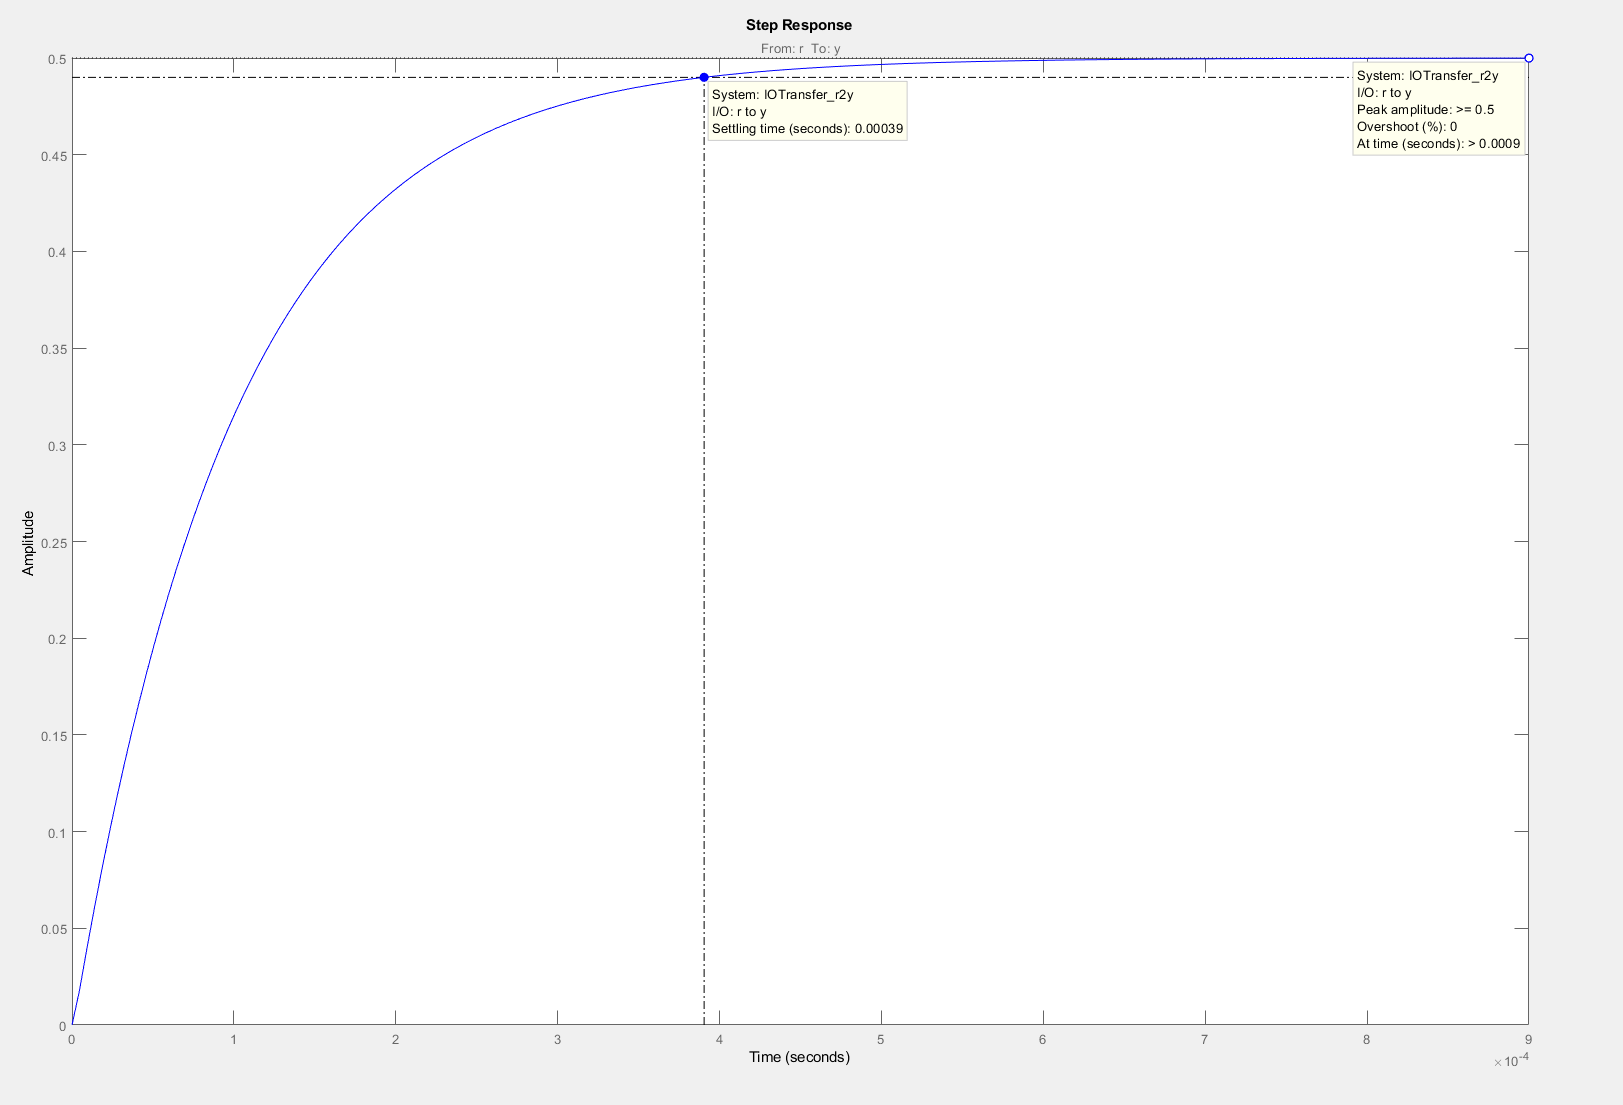
\includegraphics[width=40em,keepaspectratio]{lugar_das_raizes_18_compensacao_requerimentos}
		\par Figura 01 - Resposta de $G(s)$ à uma função degrau
	\end{center}

	% 
	% COMPENSADOR 1
	%
	\section{Compensador por Avanço de Fase}
	\paragraph{Objetivo} Deseja-se um Compensador por Avanço de Fase $C_A$ que altere o desempenho da planta, tal que $\hat{M_p} = 0.2$ e $\hat{T_s} = \SI{0.0003}{\second}$
	
	\vspace{0.5em}
	\subsection{Encontrando $\hat{w_n}$ e $\hat{\xi}$}
	\begin{align}
	\hat{M_p} &= e^{\frac{-\pi\hat{\xi}}{\sqrt{1-\hat{\xi}^2}}} \\
	0.2 &= e^{\frac{-\pi\hat{\xi}}{\sqrt{1-\hat{\xi}^2}}} \\
	ln(0.2) &= \frac{-\pi\hat{\xi}}{\sqrt{1-\hat{\xi}^2}} \\
	(-1.61)^2 &= \frac{\pi^2\hat{\xi}^2}{1-\hat{\xi}^2} \\
	\hat{\xi}^2(\pi^2+2.59) &= 2.59\\
	\hat{\xi}&= 0.488
	\end{align}  
	
	\vspace{0.5em}
	\begin{align}
	\hat{T_s} &= \frac{4}{\hat{\xi} \hat{w_n}} \\
	0.0003 &= \frac{4}{0.488\hat{w_n}} \\
	\hat{w_n} &= 27 313.12
	\end{align}
	
	\subsection{Polo Dominante do Compensador ($\hat{p}$)}
	\begin{align}
	\hat{p} &= -\hat{w_n}\pm jw_n\sqrt{1-\xi^2}\\
	\hat{p} &= -13333.334 \pm j23837.55
	\end{align}
	\vspace{0.5em}
	
	\subsection{Contribuição Angular de $\hat{p}$}
	
	\begin{align}
	\phase{G(s)*G_{C_A}(s)}_{s=\hat{p}} &= \pm\ang{180}(2k+1) & k=0,1,2...  \\
	\phase{G_{C_A}(s)}_{s=\hat{p}}+\phase{G(s)}_{s=\hat{p}}&= \ang{180} & k=0
	\end{align}
	\vspace{0.5em}
	\begin{align}
		\phase{G(s)}_{s=\hat{p}} &= \phase{\frac{1}{2\times10^{-10}s^2+0.0002011s+1}}_{s=\hat{p}} \\
		\phase{G(s)}_{s=\hat{p}} &= \phase{1}_{s=\hat{p}}- \phase{2\times10^{-10}s^2}_{s=\hat{p}}- \phase{0.0002011s}_{s=\hat{p}}-\phase{1}_{s=\hat{p}} \\			
		\phase{G(s)}_{s=\hat{p}} &=- \phase{2\times10^{-10}s^2}_{s=\hat{p}}- \phase{0.0002011s}_{s=\hat{p}}\\
		\phase{G(s)}_{s=\hat{p}} &=- \phase{2\times10^{-10}*(-13333.334 + j23837.55)}- \phase{0.0002011*(-13333.334 + j23837.55)}\\
		\phase{G(s)}_{s=\hat{p}} &=-\ang{110.65}
	\end{align}
	\vspace{0.5em}
	\par Substituindo $(43)$ em $(38)$:
	\begin{align}
	\phase{G_{C_A}(s)}_{s=\hat{p}}-\ang{110.65} &= \ang{180} \\
	\phase{G_{C_A}(s)}_{s=\hat{p}} &= \ang{290.65}
	\end{align}
	\vspace{0.5em}
	\par Um Compensador por Avanço de Fase consegue alterar a fase entre $\ang{0}$ e $\ang{90}$. Contudo, $\phase{G_{C_A}(s)}_{s=\hat{p}} = \ang{290.65} > \ang{90}$. Serão necessários quatro Compensadores por Avanço de Fase para que os requisitos sejam atendidos.
	
	\subsection{1º Compensador por Avanço de Fase}
	\par A Função de Transferência em Malha Fechada $G(s)$ possui dois polos $p_1=-4997.5$ e $p_2=-1000502.47$ e nenhum zero. Conforme mostra a Figura 2, o lugar das raízes não passa pelo polo dominante $\hat{p}$ desejado, o que mostra ser impossível ajustar o funcionamento da planta somente com variação do ganho, sendo necessário um Compensador.
	\begin{center}
	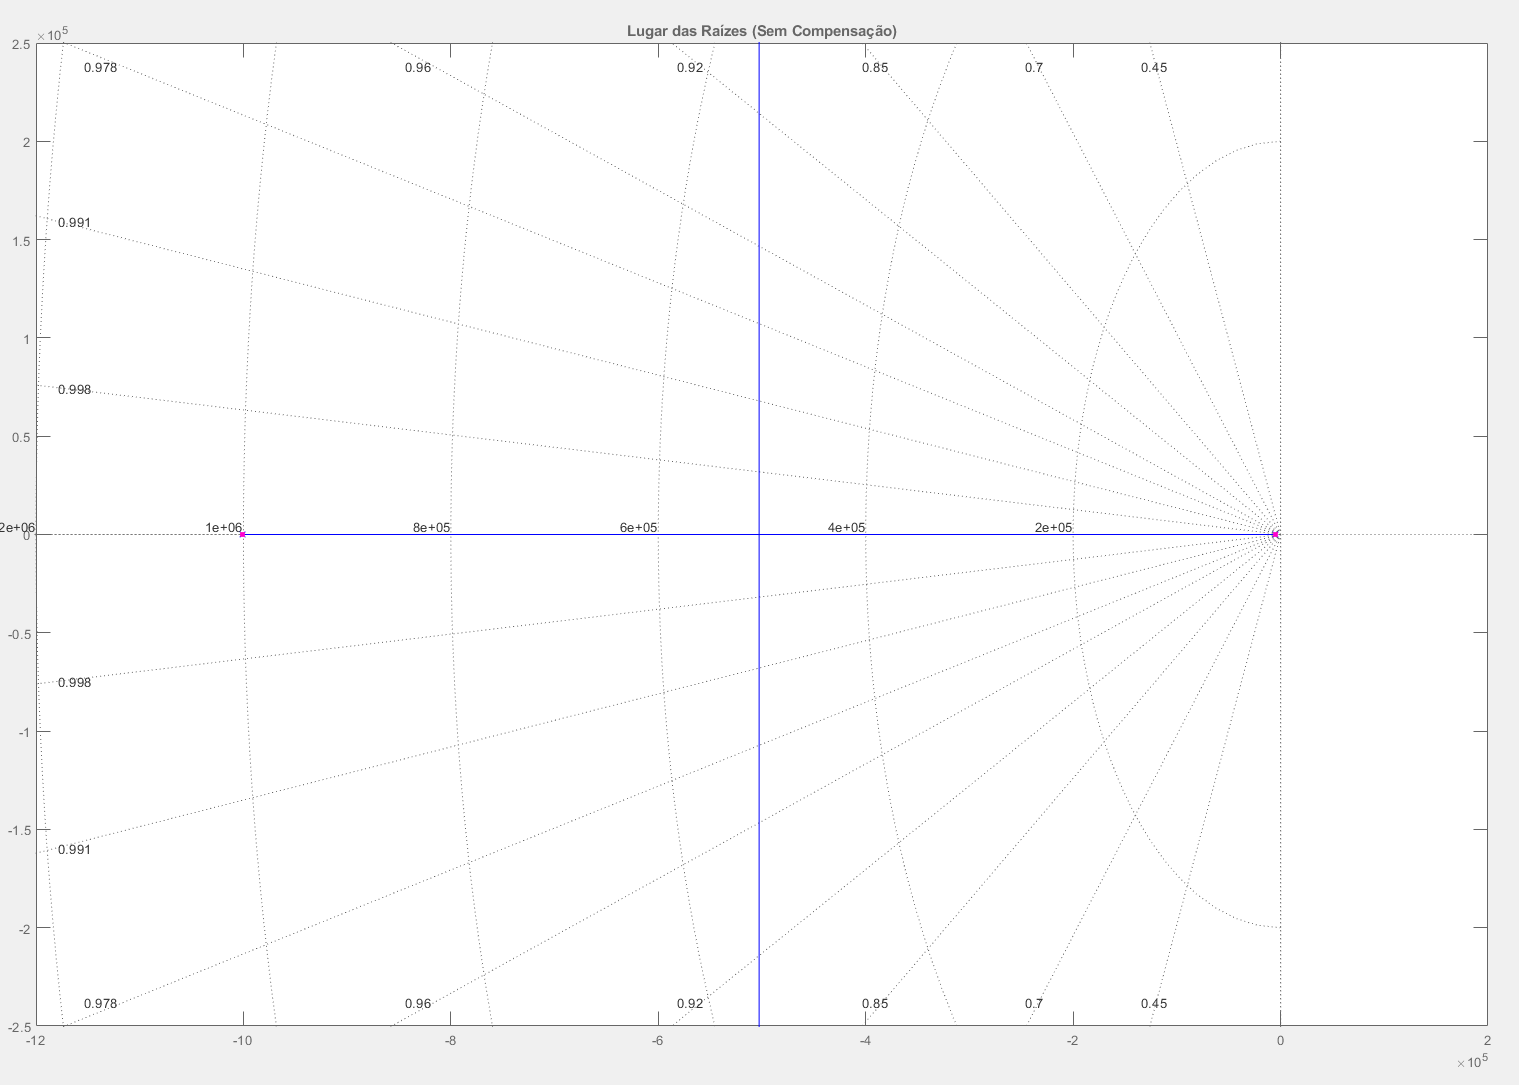
\includegraphics[width=40em,keepaspectratio]{lugar_das_raizes_sem_compensacao}
	\par Figura 02 - Lugar das Raízes sem Compensação
	\end{center}
	
	\vspace{0.5em}
	\par Nesta primeira compensação, deseja-se gerar um avanço de fase de $\ang{72.66}$, que corresponde a um quarto do avanço de fase desejado.
	\vspace{0.5em}
	\par Sendo a equação que define um Compensador por Avanço de Fase $G_{C_A}$:
	\begin{align}
		G_{C_A} &= K_c * \frac{s+\frac{1}{T_1}}{s+\frac{\gamma}{T_1}}
	\end{align}
	\vspace{0.5em}
	\par Deseja-se calcular os parâmetros $T_1$, $K_c$ e $\gamma$. Contudo, para tal, é necessário antes encontrar as raízes do Compensador para se garantir o efeito desejado, i.e., um avanço de $\ang{72.66}$ na fase.
	\vspace{0.5em}
	\par O Zero do Compensador $Z_{C_1}$ será posicionado em $s=-10000$. O Polo do Compensador $P_{C_1}$ será calculado à partir de $Z_{C_1}$.
	
	\begin{align}
		\alpha &= \frac{\phase{G_{C_A}}}{4} = \ang{72.66}\\
		\alpha &= \alpha_1 + \alpha_2
	\end{align}
	\vspace{0.5em}
	\par Onde $\alpha_1$ é o ângulo entre ${\hat{p}}$ e $P_{C_1}$ e $\alpha_2$ é o ângulo entre ${\hat{p}}$ e ${Z_{C_1}}$.
	\vspace{0.5em}
	\begin{align}
		\alpha_2 &= \frac{tan({Z_{C_1}}-real({\hat{p}}))}{imag({\hat{p}})} \\
		\alpha_2 &= \ang{8.06}
	\end{align}
	
	\par Substituindo $(50)$ em $(48)$:
	\begin{align}
	\ang{72.66} &= \alpha_1 + \ang{8.06} \\
	\alpha_1 &= \ang{64.59}
	\end{align}
	\vspace{0.5em}
	
	\par Pode-se então calcular ${P_C}$
	\begin{align}
		P_C &= -tan(\alpha_1)*imag({\hat{p}})-real({\hat{p}}) \\
		P_C &= -63534.67
	\end{align}
 	\vspace{0.5em}
 	
 	\par Agora é possível calcular $T_1$ e $\gamma$:
 	\begin{align}
 	Z_C &=\frac{1}{T_1} \\
 	T_1 &= 10^{-4}
 	\end{align}
 	\vspace{0.5em}
 	\begin{align}
 	P_C &=\frac{\gamma}{T_1} \\
 	\gamma &= 6.353
 	\end{align}
 	
 	\vspace{0.5em}
 	\par Sabendo que:
 	\begin{align}
	|K_c*G_{C_1}(s)*G(s)|_{s=\hat{p}} &=1 \\
	K_C &= |\frac{1}{G_{C_1}(s)*G(s)}|_{s=\hat{p}} \\
	K_C &= |\frac{s+63534.67}{s+10000} *(2\times10^{-10})*\frac{(s+1000502.47)(s+4997.5)}{1} |_{s=\hat{p}} \\
	K_C &= 11.515
 	\end{align}
 	
 	\vspace{0.5em}
 	\par Portanto, temos formada a Função de Transferência do Primeiro Compensador, ao substituirmos $(56)$, $(58)$ e $(62)$ em $(46)$:
 	\begin{align}
 	G_{C_1} &= 11.515 * \frac{s+10000}{s+63534.67}
 	\end{align}
 	\vspace{0.5em}
 	\par Na Figura 03 é possível observar a influência de ${P_{C_1}}$ e $Z_{C_1}$ no Lugar das Raízes:
	\begin{center}
 		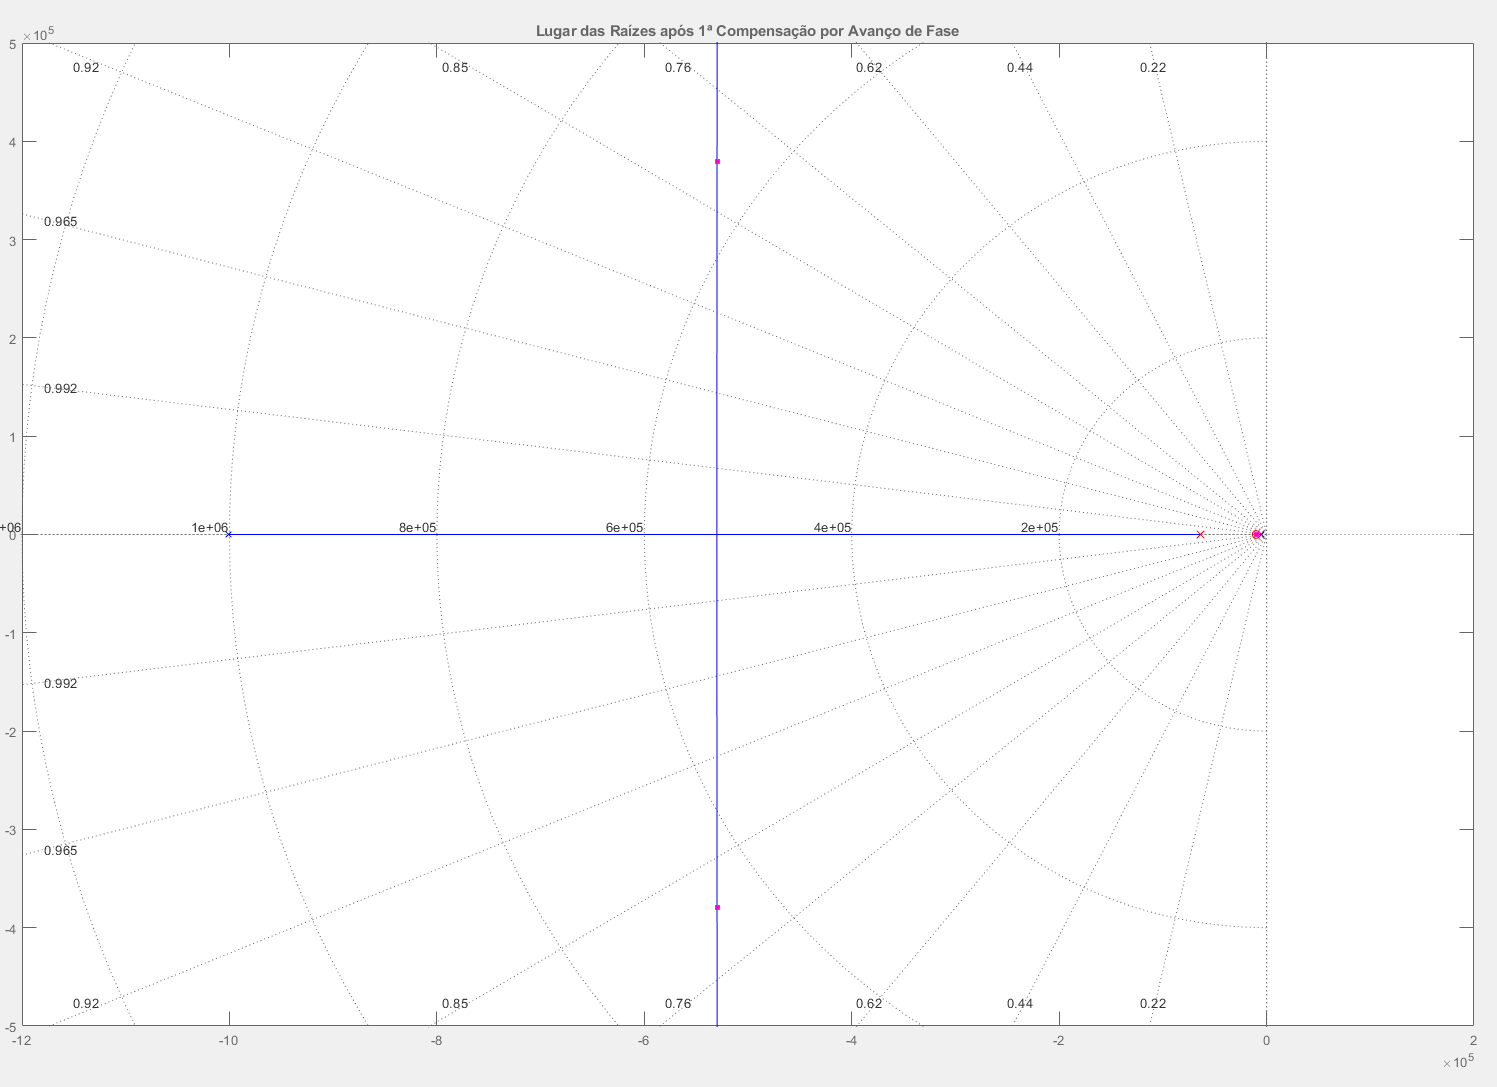
\includegraphics[width=40em,keepaspectratio]{lugar_das_raizes_1_compensacao}
 		\par Figura 03 - Lugar das Raízes após a 1ª Compensação por Avanço de Fase
 	\end{center}
 
 \subsection{Demais Compensadores por Avanço de Fase}
 \par O Compensador $C_1$ foi projetado de modo que o avanço na fase da Planta seja de $\frac{1}{4}$ do avanço total necessário. Deste modo, basta inserir outros três compensadores $C_2$, $C_3$ e $C_4$ idênticos a $C_1$ para que o Lugar das Raízes atinja os requisitos desejados. As Figuras 04, 05 e 06 mostrarão a influência da adição de cada um dos compensadores no Lugar das Raízes do Sistema.

\begin{center}
	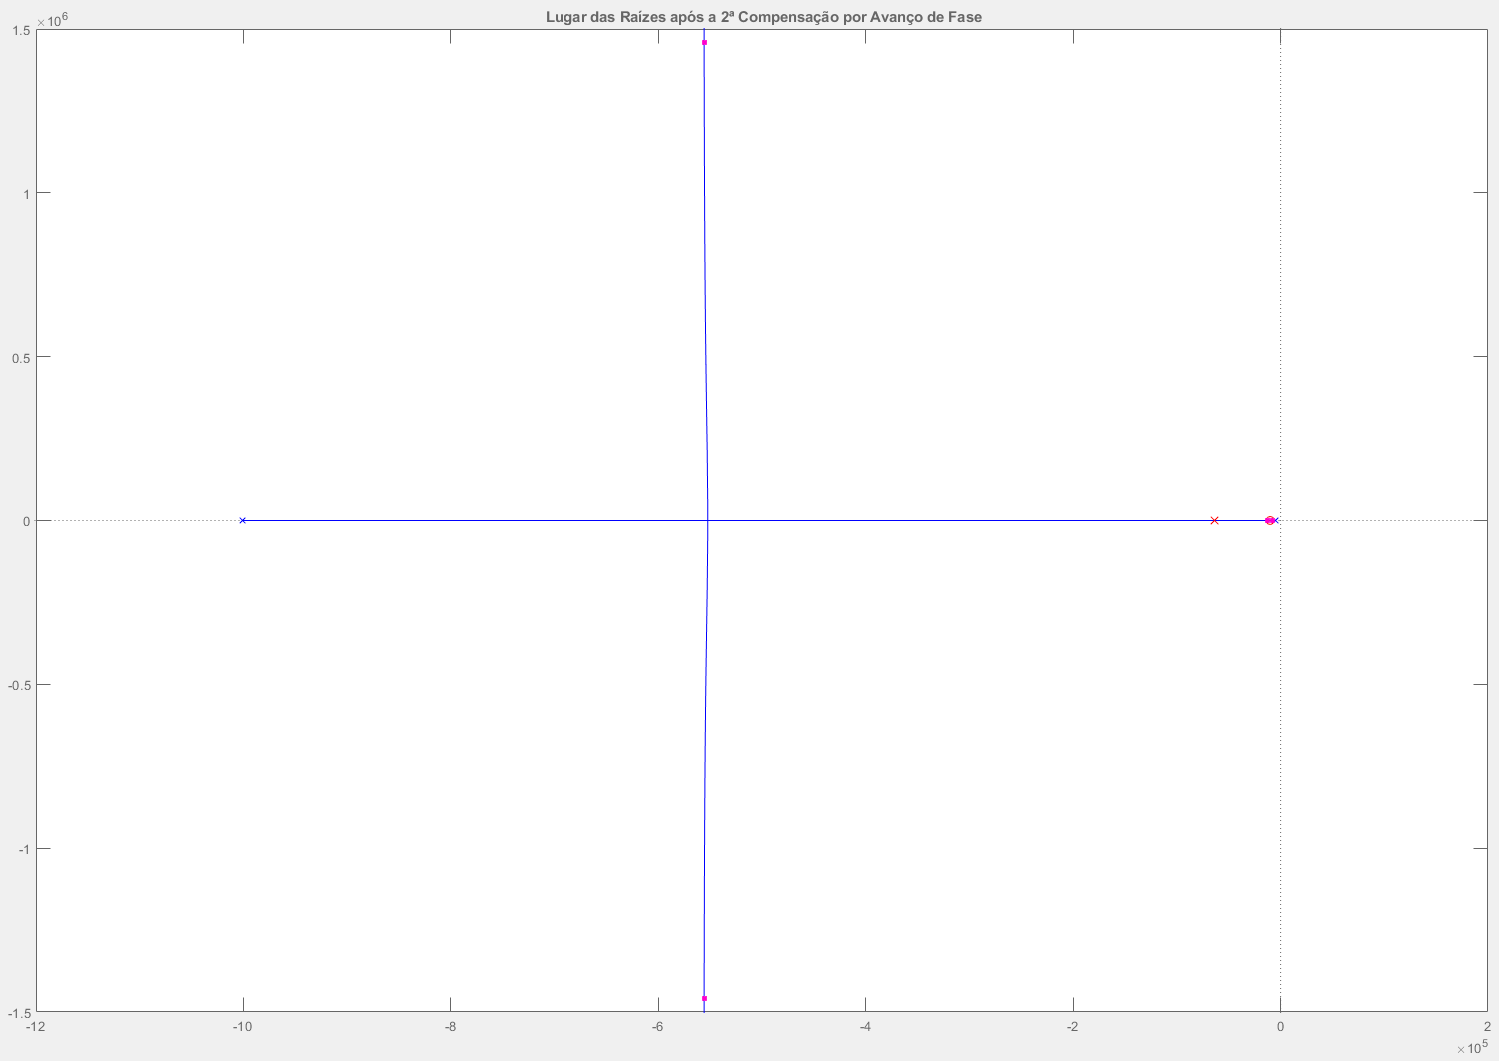
\includegraphics[width=40em,keepaspectratio]{lugar_das_raizes_12_compensacao_requerimentos}
	\par Figura 04 - Lugar das Raízes após a 2ª Compensação por Avanço de Fase
\end{center}
 
 \begin{center}
 	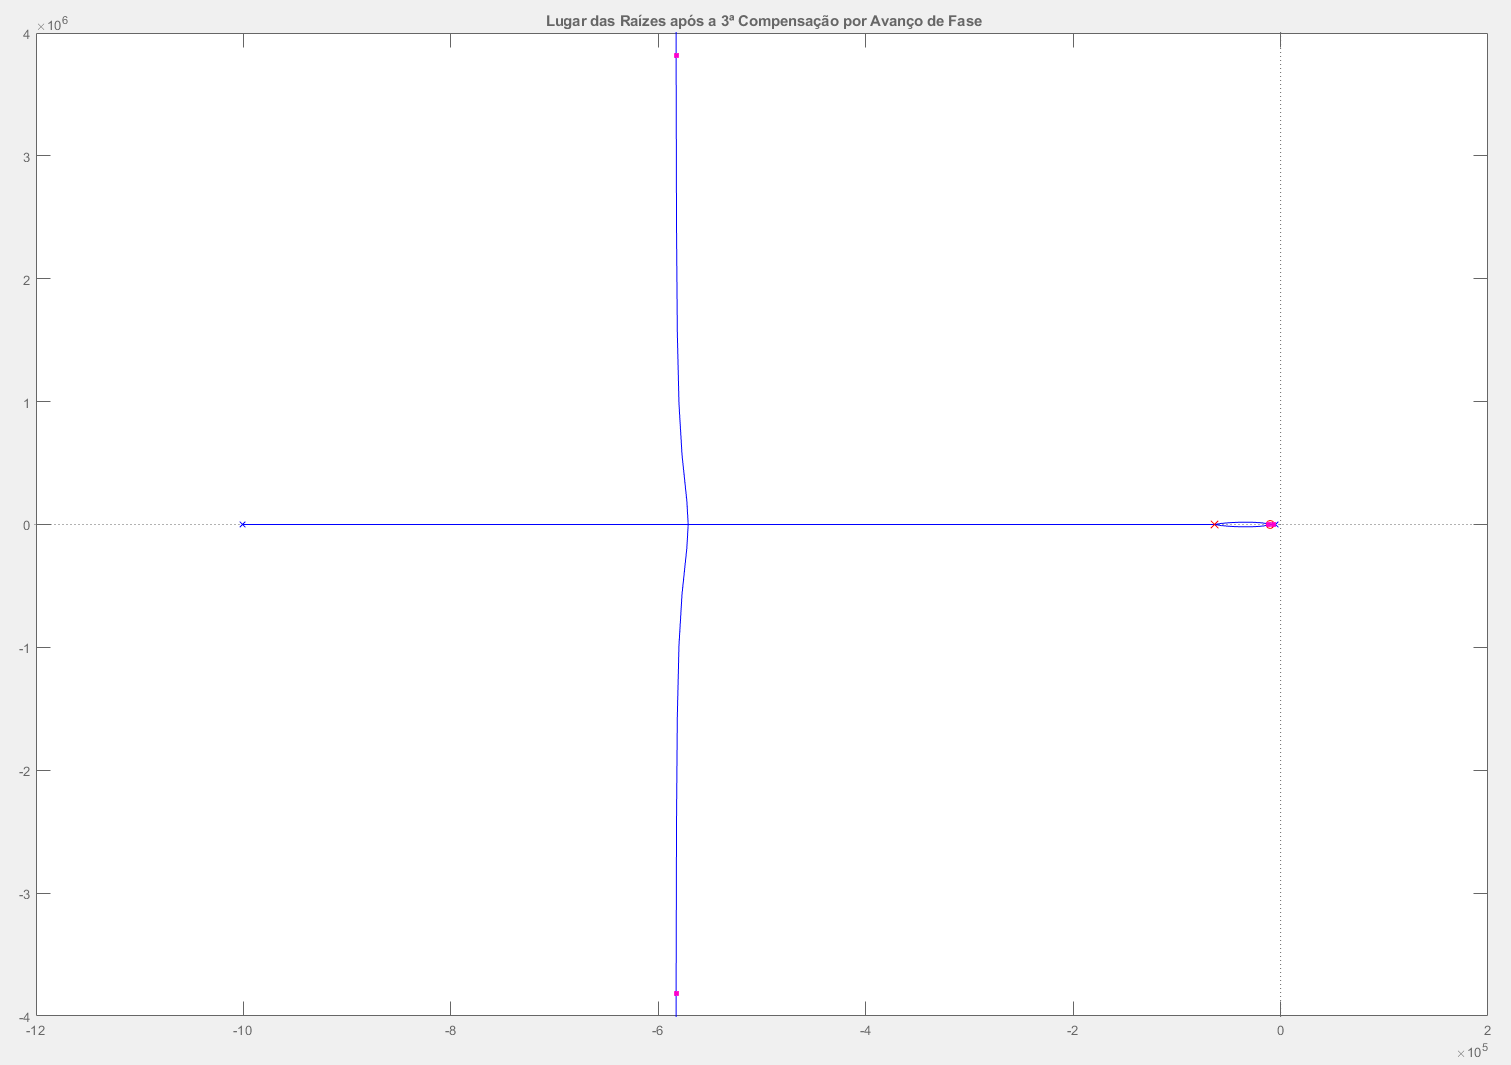
\includegraphics[width=40em,keepaspectratio]{lugar_das_raizes_13_compensacao_requerimentos}
 	\par Figura 05 - Lugar das Raízes após a 3ª Compensação por Avanço de Fase
 \end{center}

 \begin{center}
	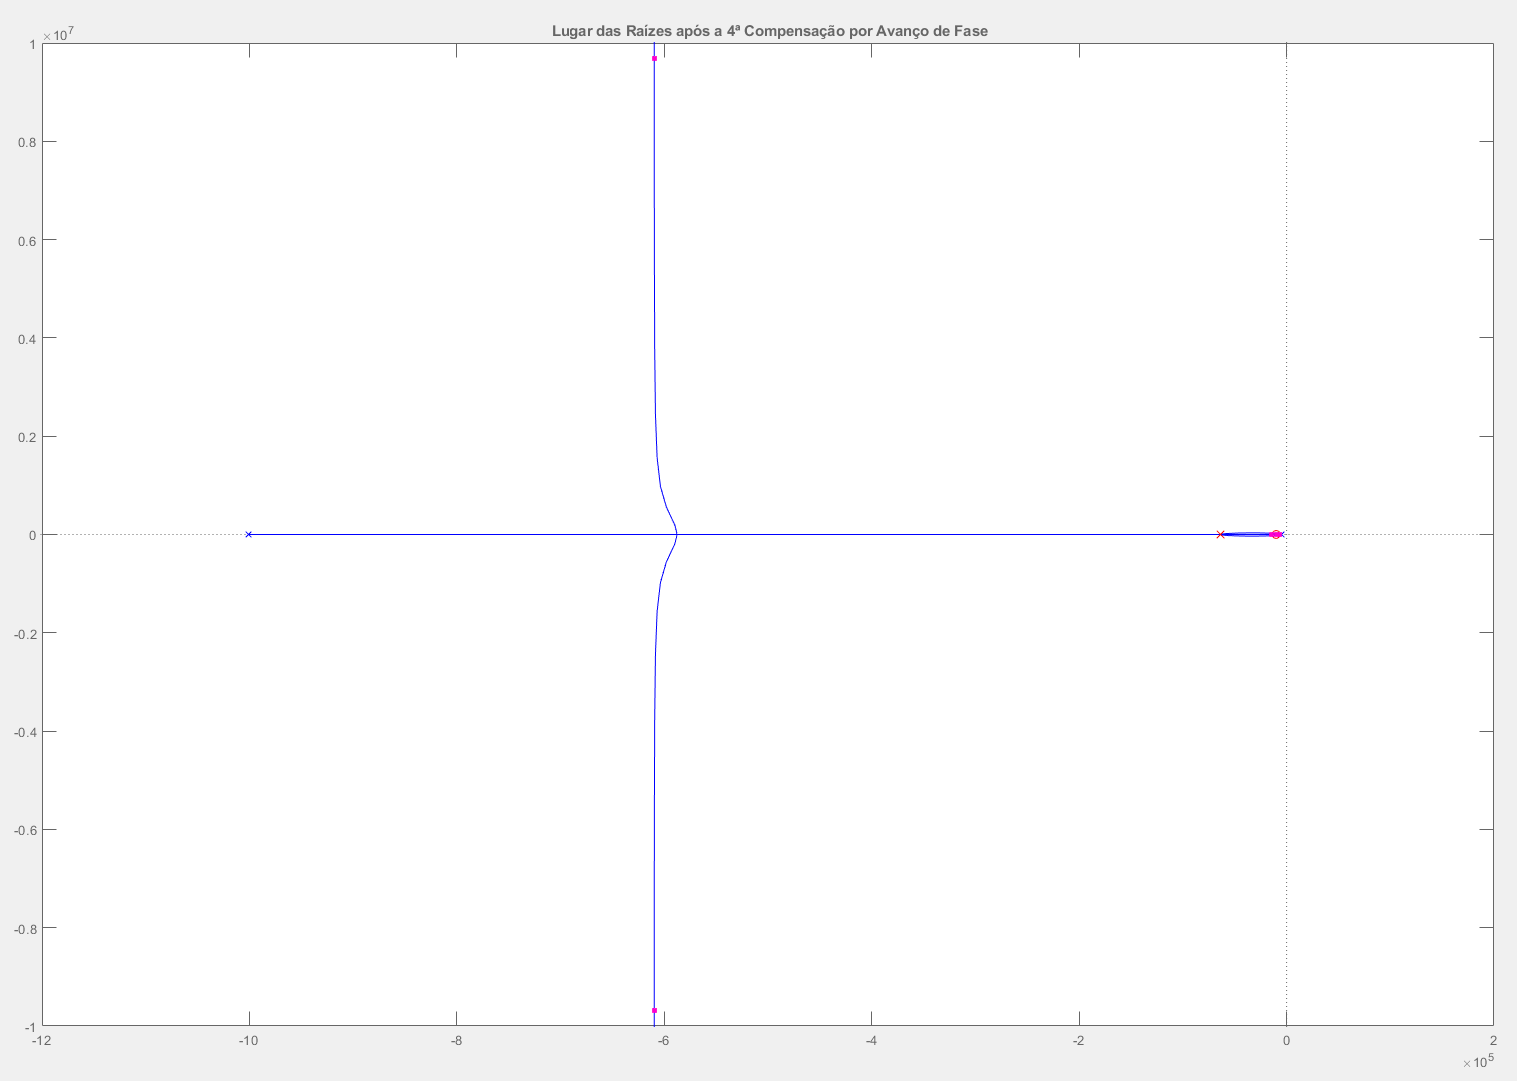
\includegraphics[width=40em,keepaspectratio]{lugar_das_raizes_14_compensacao_requerimentos}
	\par Figura 06 - Lugar das Raízes após a 4ª Compensação por Avanço de Fase
 \end{center}

 \subsection{Avaliação da Compensação por Avanço de Fase}
 \par A Figura 07 demonstra como o Lugar das Raízes após a 4ª Compensação por Avanço de Fase se comporta ao ser comparado com os Requerimentos $M_p = 0.2$ e $T_s = \SI{0.0003}{\second}$. Entretanto a Figura 09 mostra que a resposta ao Impulso não é a esperada, sendo o Tempo de Resposta Real em torno de $\SI{6}{\micro\second}$ e o Máximo de Sobressinal de aproximadamente $100\%$
 \begin{center}
 	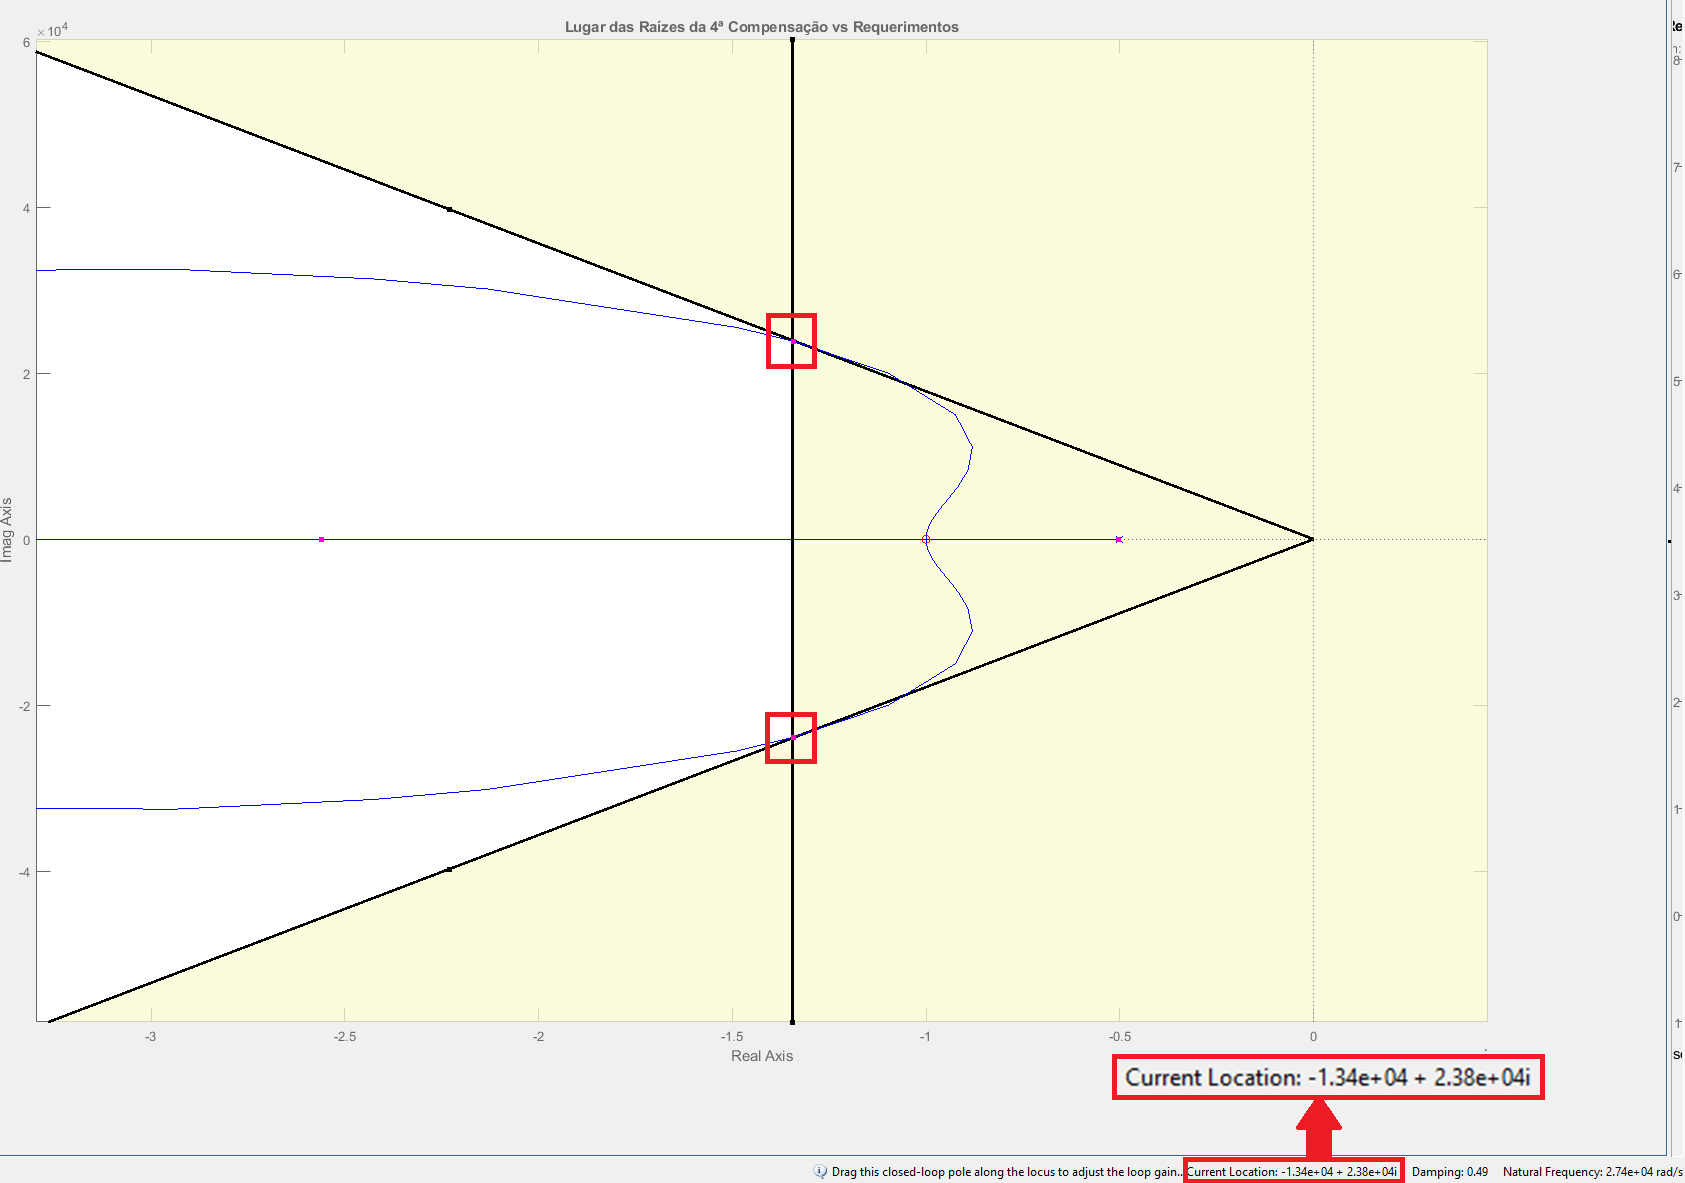
\includegraphics[width=40em,keepaspectratio]{lugar_das_raizes_1_compensacao_requerimentos}
 	\par Figura 07 - Lugar das Raízes vs. Requerimentos após a 4ª Compensação por Avanço de Fase
 \end{center}
\begin{center}
	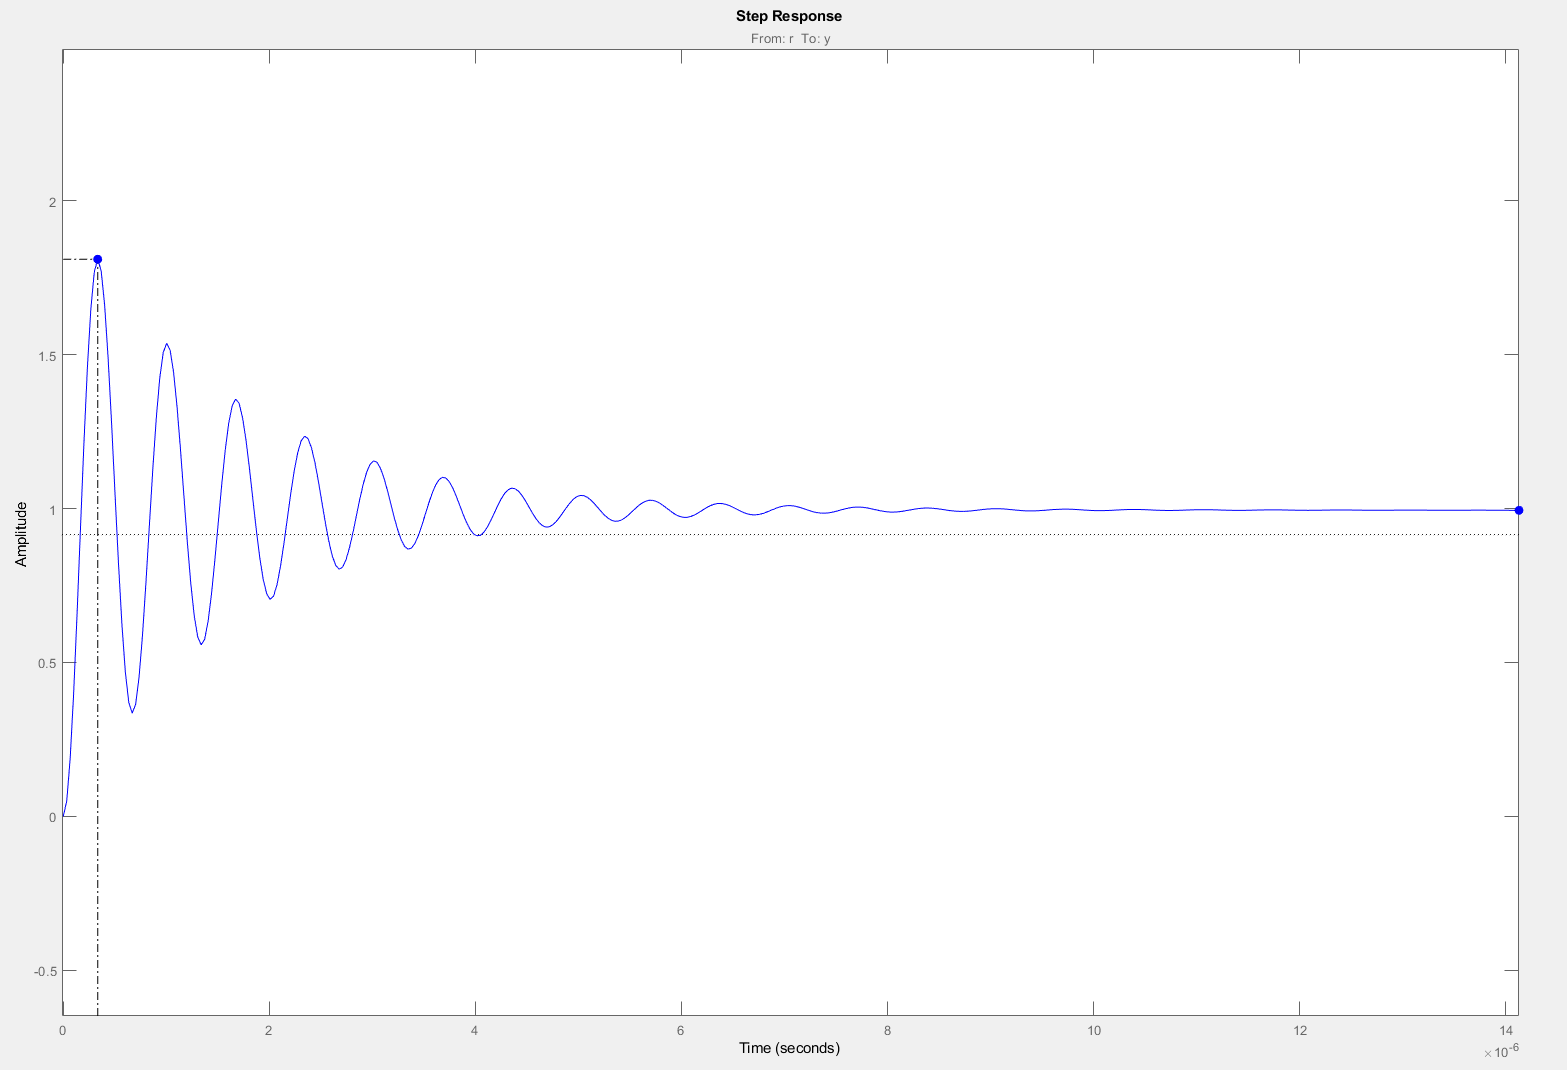
\includegraphics[width=40em,keepaspectratio]{lugar_das_raizes_19_compensacao_requerimentos}
	\par Figura 08 - Resposta de $K_c^4G_{C_A}^4(s)G(s)$ à uma função degrau
\end{center}
\vspace{0.5em}
 \vspace{0.5em}
 
 \section{Compensador por Atraso de Fase}
 \paragraph{Objetivo} Deseja-se um Compensador por Atraso de Fase $C_B$ que altere o desempenho da planta, tal que $\hat{K_v} = 100s^{-1}$
 \par Antes de realizar a modelagem do Compensador, verifica-se se o Erro Estacionário de Velocidade $K_v$ não atende ao requisito.
 \begin{align}
 K_v &= \lim_{s \to 0} sG_{C_A}(s)G(s) \\
 K_v &= \lim_{s \to 0} s\times11.515^4 \times \frac{(s+10000)^4}{(s+63534.67)^4}\times\frac{1}{2\times10^{-10}}\times\frac{1}{s^2 + 1.0055\times10^{6}s+5\times10^9} \\
 K_v &= 0\times11.515^4 \times \frac{10000^4}{63534.67^4}\times\frac{1}{2\times10^{-10}}\times\frac{1}{5\times10^9}\\
 K_v &= 0
 \end{align}
 \vspace{0.5em}
 \par Observando que o $K_v = 0s^{-1}$, é demonstrada a necessidade de um Compensador por Atraso de Fase, 
 \subsection{1º Compensador por Atraso de Fase}
 \par Sendo a equação que define um Compensador por Atraso de Fase $G_{C_B}$:
 \begin{align}
 G_{C_B} &= \frac{s+\frac{1}{T_2}}{s+\frac{1}{\beta T_2}}
 \end{align}
  \vspace{0.5em}
 \par Deseja-se calcular os parâmetros $T_2$ e $\beta$. Para isso, multiplica-se $(64)$ por $(68)$ e substitui-se ${K_v}$ por $\hat{K_v}$:
 \begin{align}
  \hat{K_v} &= \lim_{s \to 0} sG_{C_A}(s)G_{C_B}(s)G(s) \\
   \hat{K_v}  &= \lim_{s \to 0} s\times11.515^4 \times \frac{(s+10000)^4}{(s+63534.67)^4}\times\frac{1}{2\times10^{-10}}\times\frac{s+\frac{1}{T_2}}{s+\frac{1}{\beta_1 T_2}}\times\frac{1}{s^2 + 1.0055\times10^{6}s+5\times10^9}
 \end{align}
 \vspace{0.5em}
\par É necessário adicionar um polo muito próximo a $s=0$ para que o Erro Estacionário de Velocidade não seja nulo. Portanto, será escolhido $T_2$ suficientemente grande de modo que $\frac{1}{\beta T_2} \to 0$.
\par Utilizando $T_2=2$, sabendo que $\beta_1 >> 1$:
 \begin{align}
	\frac{1}{1\beta_1}& << 1 \\
	\frac{1}{1\beta_1}&\approx 0 & \forall \beta_1  : \beta_1 >> 1
\end{align}
\vspace{0.5em}
\par Utilizando $\beta_1=10000$:
\begin{align}
\hat{K_v}  &= \lim_{s \to 0} s\times11.515^4 \times \frac{(s+10000)^4}{(s+63534.67)^4}\times\frac{1}{2\times10^{-10}}\times\frac{s+\frac{1}{20000}}{s}\times\frac{1}{s^2 + 1.0055\times10^{6}s+5\times10^9} \\
\hat{K_v} &= 11.515^4 \times \frac{(10000)^4}{(63534.67)^4}\times\frac{1}{2\times10^{-10}}\times\frac{1}{20000}\times\frac{1}{5\times10^9} \\
\hat{K_v} &= 5.39
\end{align}
\paragraph{Observação} Deste modo não será possível regular $\beta_1$ com a intenção de se atingir o Erro Estacionário desejado, sendo necessário um 2º Compensador por Atraso de Fase.
 \subsection{Avaliação do 1º Compensador por Atraso de Fase}
 \par Um Compensador por Atraso de Fase possui certas limitações, para que o Lugar das Raízes não seja alterado. Portanto, são necessárias duas análises:
\begin{align}
	\phase{G_{C_5}}_{s=\hat{p}} &< \ang{5} 
	\\
	|G_{C_5}|_{s=\hat{p}} &= 1
\end{align}

\vspace{0.5em}

\begin{align}
\phase{G_{C_5}}_{s=\hat{p}} &< \ang{5} \\
\phase{\frac{s+\frac{1}{20000}}{s}}_{s=\hat{p}} &< \ang{5}  \\
\phase{\frac{s+\frac{1}{20000}}{s}}_{s=\hat{p}} =\ang{-0.00009} &< \ang{5} 
\end{align}
\vspace{0.5em}
\begin{align}
|G_{C_5}|_{s=\hat{p}} &= 1 \\
|\frac{s+\frac{1}{8000}}{s}|_{s=\hat{p}} &= 1  \\
|\frac{s+\frac{1}{8000}}{s}|_{s=\hat{p}} = 0.9999 &\approx 1  
\end{align}
\vspace{0.5em}
\par O 1º Compensador por Atraso de Fase atende aos requisitos. Na Figura 09 é comprovado que o Lugar das Raízes não foi alterado.
\begin{center}
	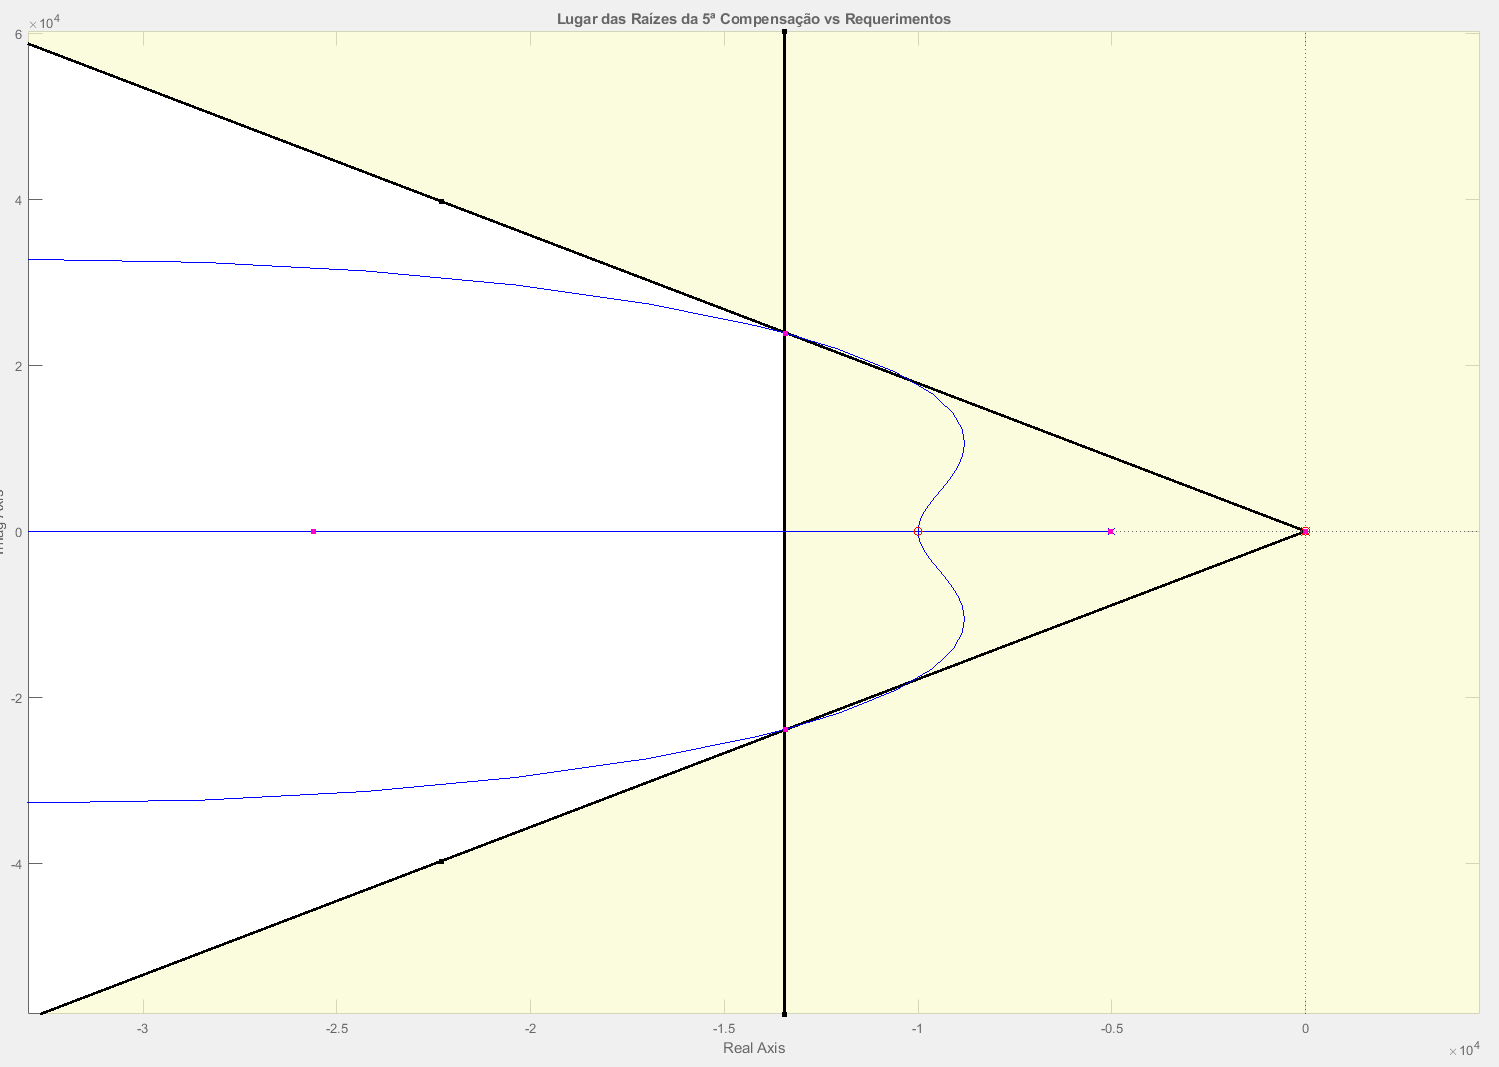
\includegraphics[width=40em,keepaspectratio]{lugar_das_raizes_15_compensacao_requerimentos}
	\par Figura 09 - Lugar das Raízes vs. Requerimentos após a 1ª Compensação por Atraso de Fase
\end{center}
\vspace{0.5em}
 \subsection{2º Compensador por Atraso de Fase}
\par Para se que a Constante de Erro de Velocidade $\hat{K_v} = 100s^{-1}$, é necessário um 2º Compensador por Atraso de Fase. A modelagem seguirá os mesmos passos que no 1º Compensador por Atraso de Fase.
 \begin{align}
\hat{K_v}  &= \lim_{s \to 0} s\times\frac{11.515^4}{2\times10^{-10}}\times \frac{(s+10000)^4}{(s+63534.67)^4}\times\frac{s+\frac{1}{20000}}{s}\times\frac{s+\frac{1}{T_3}}{s+\frac{1}{\beta_2 T_3}}\times\frac{1}{s^2 + 1.0055\times10^{6}s+5\times10^9} \\
100 &= \frac{11.515^4}{2\times10^{-10}}\times \frac{(10000)^4}{(63534.67)^4}\times\frac{1}{20000}\times\frac{1}{5\times10^9} \times\lim_{s \to 0} \frac{s+\frac{1}{T_3}}{s+\frac{1}{\beta_2 T_3}}\\
100 &= 0.706\times\lim_{s \to 0} \frac{s+\frac{1}{T_3}}{s+\frac{1}{\beta_2 T_3}}
\end{align}
\vspace{0.5em}
\par Usando $T_3=0.1$:
  \begin{align}
 100 &= 5.39\times \lim_{s \to 0}\frac{s+\frac{1}{T_3}}{s+\frac{1}{\beta_2 T_3}} \\
 100 &= 5.39\times \lim_{s \to 0}\frac{s+\frac{1}{0.1}}{s+\frac{1}{0.1	\beta_2}} \\
 100 &= 5.39\times\frac{\frac{1}{0.1}}{\frac{1}{0.1\beta_2}}\\
 \beta_2 &= \frac{100}{5.39} \\
 \beta_2 &= 18.53
 \end{align}
 \par Deste modo:
  \begin{align}
 G_{C_6} &= \frac{s+10}{s+0.53}
 \end{align}
 \begin{align}
 \phase{\frac{s+10}{s+0.53}}_{s=\hat{p}} = \ang{-0.017} &< \ang{5}
 \end{align}
 \vspace{0.5em}
 \begin{align}
|\frac{s+10}{s+0.53}|_{s=\hat{p}} = 0.998 &\approx 1  
\end{align}
 \par Sendo assim, ${G_{C_6}}$ atinge o objetivo desejado, e atinge os Requisitos, como mostra a Figura 09. 

\begin{center}
	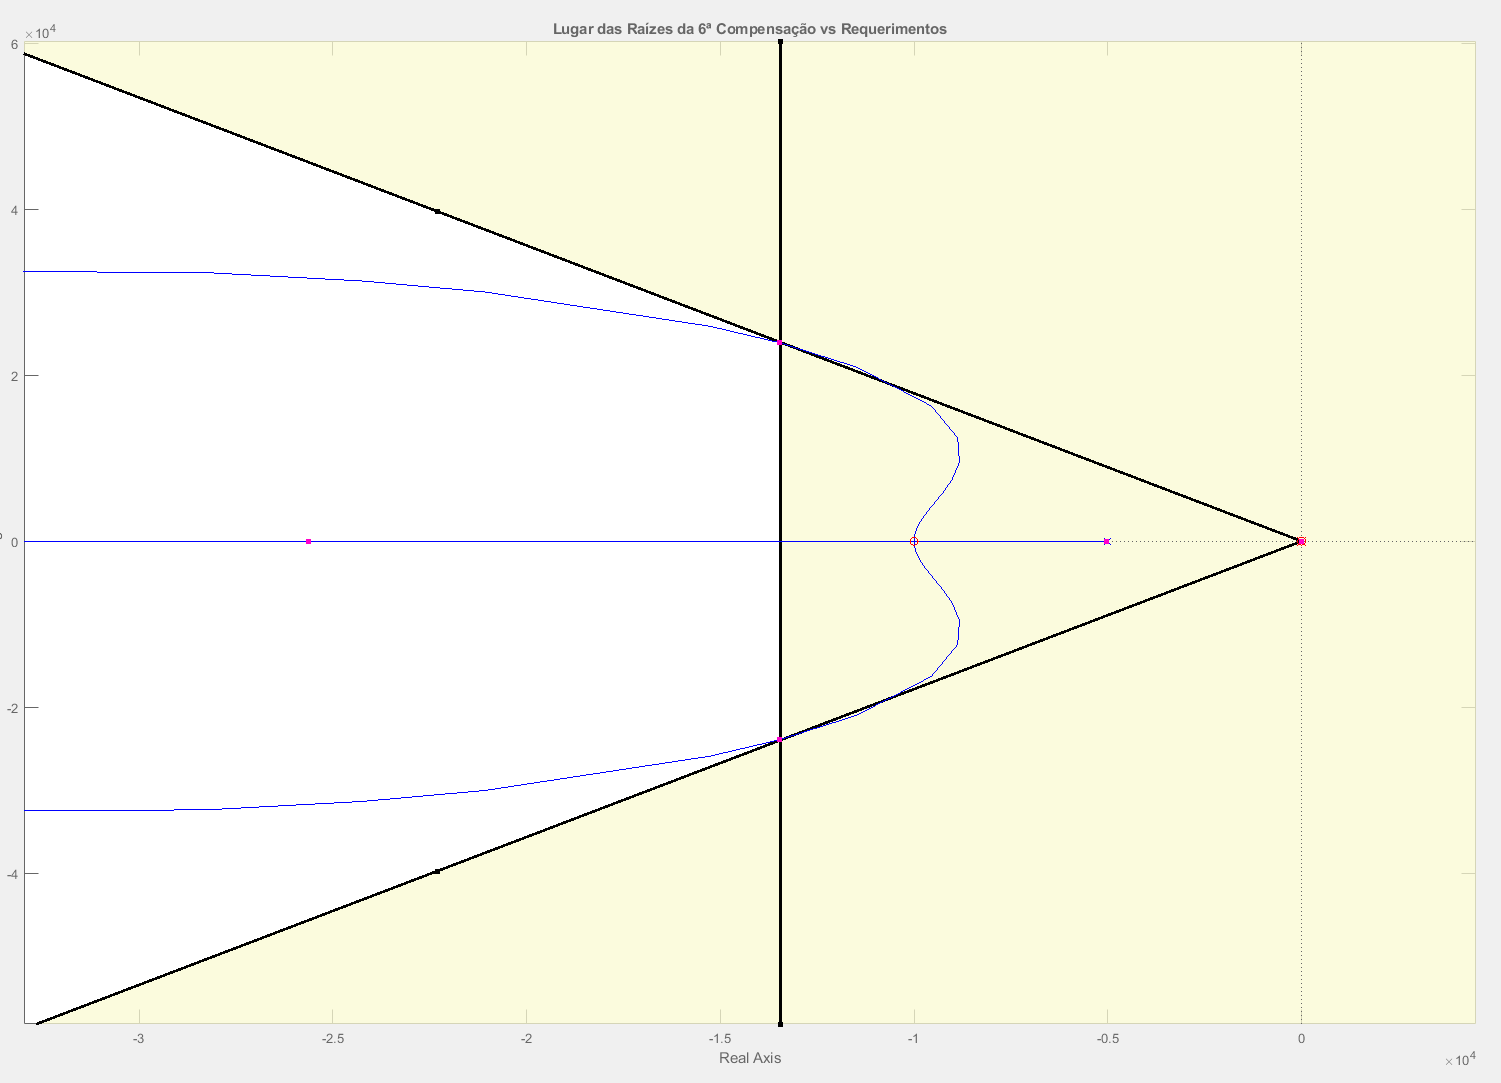
\includegraphics[width=35em,keepaspectratio]{lugar_das_raizes_16_compensacao_requerimentos}
	\par Figura 09 - Lugar das Raízes vs. Requerimentos após a 2ª Compensação por Atraso de Fase
\end{center}
	\vspace{0.5em} 
	\par Entretanto, ao se simular uma entrada em degrau, o Sistema não mostra a resposta prevista: $M_p = 81.1\%$ e $T_s=\SI{6.73}{\micro\second}$. Isto pode ser explicado pela aproximação de valores e pela diferença de ordens de grandeza das variáveis utilizadas. 
\begin{center}
	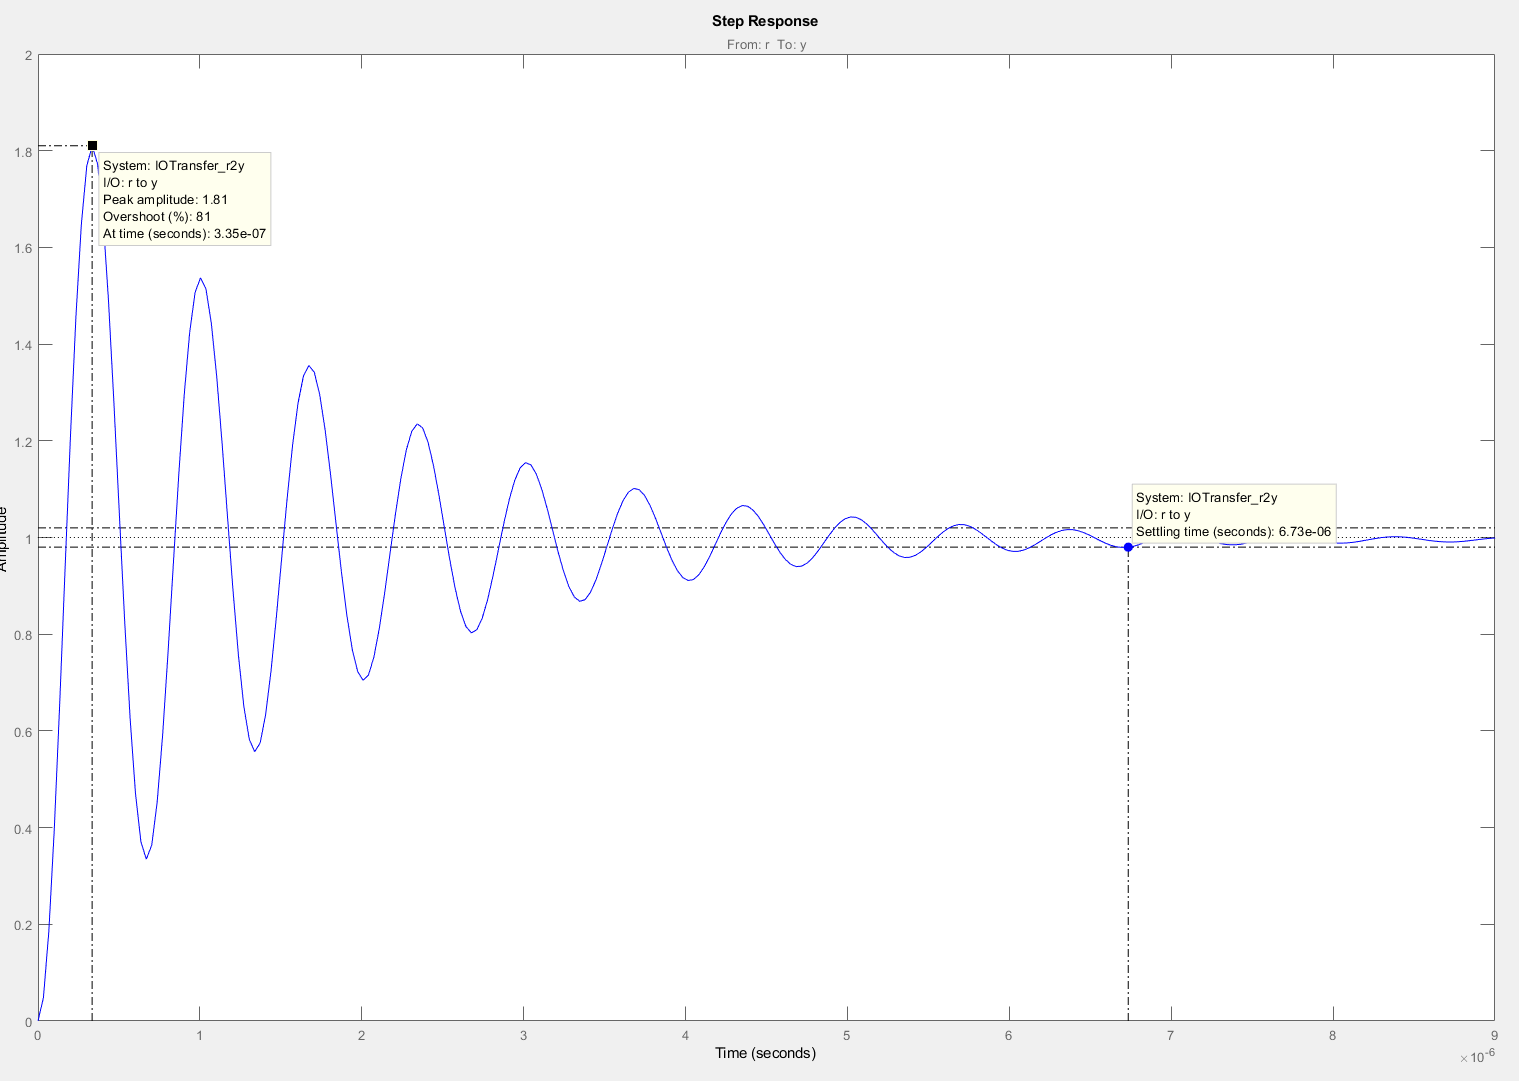
\includegraphics[width=35em,keepaspectratio]{lugar_das_raizes_17_compensacao_requerimentos}
	\par Figura 09 - Resposta de $K_c^4G_{C_A}^4(s)G_{C_B}(s)G_{C_C}(s)G(s)$ à uma função degrau
\end{center}
\par Após a Compensação, o Sistema se mostra mais rápido e menos amortecido que o Sistema antes da compensação, mostrado na Figura 01.

\section{Modelo de Circuito}
\par Será utilizado o Modelo de Compensadores por Avanço-Atraso de Fase mostrado na Figura 10
\begin{center}
	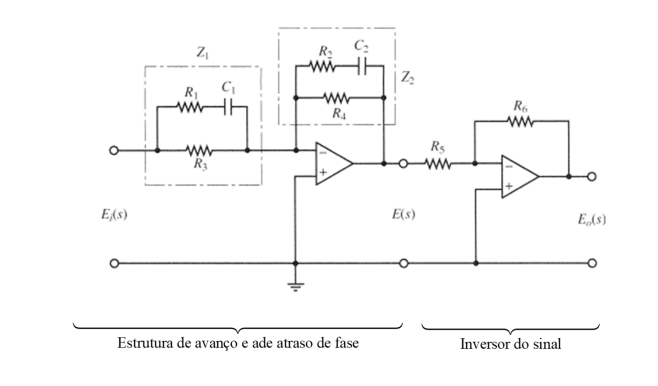
\includegraphics[width=35em,keepaspectratio]{circuito}
	\par Figura 10 -  Modelo de Compensadores por Avanço-Atraso de Fase
\end{center}
\par Sabendo que:
\begin{align}
	T_1 &= (R_1+R_3)C_1 \\
	\gamma &= \frac{R_1+R_3}{R_1} \\
	T_2 &= R_2C_2 \\
	\beta &= \frac{R_2+R_4}{R_2} \\
	K_C &= \frac{R_2R_4R_6}{R_1R_3R_5} \frac{R_1+R_3}{R_2+R_4}
\end{align}
\subsection{Cálculo dos Componentes para o Compensador por Avanço de Fase}
\par Todos os quatro Compensadores por Avanço de Fase são iguais, logo utilizam os mesmo componentes.  Sendo as características do Capacitor por Avanço de Fase:
\begin{align}
	T_1&=10^{-4}\\
	\gamma&=6.353
\end{align}
\par Substituindo $(100)$ e $(101)$ em $(95)$ e $(96)$, e usando $C_1=\SI{10}{\nano\farad}$:
\begin{align}
	10^{-4} &= (R_1+R_3)\times \SI{10}{\nano\farad}\\
	\frac{10^{-4}}{10\times10^{-9}} &= R_1+R_3 \\
	R_1+R_3  &= 10^4
\end{align}
	\vspace{0.5em}
\begin{align}
	6.353 &= \frac{R_1+R_3}{R_1} \\
    R_1 &= \frac{10^4}{6.353} \\
	R_1 &\approx \SI{1.5}{\kilo\ohm}
\end{align}
\vspace{0.5em}
\begin{align}
1.5\times10^3+R_3  &= 10^4\\
R_3  &\approx \SI{8.5}{\kilo\ohm}
\end{align}
\subsection{Cálculo dos Componentes para o Compensador por Atraso de Fase}
\par Temos dois Compensadores por Atraso de Fase distintos, cujo os dados são:
\begin{align}
	T_2 &= 2\\
	\beta_1 &= 10000\\
	T_3 &= 0.2\\
	\beta_2 &= 18.53
\end{align}
\vspace{0.5em}
\par Para o 1º Compensador por Atraso de Fase:
\par Substituindo$(110)$ e $(111)$ em $(97)$ e $(98)$, e usando $C_2  =\SI{1}{\milli \farad}$:
\begin{align}
R_2 &= \frac{2}{10^{-3}}\\
R_2 &\approx \SI{2}{\kilo\ohm}\\
\end{align}
\vspace{0.5em}
\begin{align}
10000 &= \frac{2\times10^3+R_4}{2\times10^3}\\
R_4 &= 2\times10^{7}-2\times10^6\\
R_4 &\approx \SI{19.998}{\mega\ohm}
\end{align}
\vspace{10em}
\par Para o 2º Compensador por Atraso de Fase:
\par Substituindo $(110)$ e $(111)$ em $(97)$ e $(98)$, e usando $C_2=\SI{1}{\micro\farad}$:
\begin{align}
R_2 &= \frac{0.2}{10^{-6}}\\
R_2 &\approx \SI{200}{\kilo\ohm}
\end{align}
\vspace{0.5em}
\begin{align}
18.53 &= \frac{200\times10^3+R_4}{200\times10^3}\\
R_4 &= 3.707\times10^{6}-2\times10^3\\
R_4 &\approx \SI{3.7}{\mega\ohm}
\end{align}
\subsection{Cálculo dos Componentes para o Ganho}
\par Como estamos utilizando seis compensadores no total, o ganho depende de todos eles. Logo, a equação para cálculo de componentes do ganho é na seguinte forma:

\begin{align}
K_C^4 &= \frac{R_{2_1}R_{4_1}R_{2_2}R_{4_2}R_6}{R_1^4R_3^4R_5} \frac{(R_1+R_3)^4}{(R_{2_1}+R_{4_1})(R_{2_2}+r_{4_2})}
\end{align}
\par Usando $R_6=\SI{100}{\kilo\ohm}$, temos:
\begin{align}
\frac{R_5}{R_6} &= \frac{R_{2_1}R_{4_1}R_{2_2}R_{4_2}}{R_1^4R_3^4}\times \frac{(R_1+R_3)^4}{(R_{2_1}+R_{4_1})(R_{2_2}+R_{4_2})}\times\frac{1}{K_C^4}\\
R_5 &= 100\times10^3\times\frac{R_{2_1}R_{4_1}R_{2_2}R_{4_2}}{R_1^4R_3^4}\times \frac{(R_1+R_3)^4}{(R_{2_1}+R_{4_1})(R_{2_2}+R_{4_2})}\times\frac{1}{K_C^4}\\
R_5 &\approx \SI{13}{\ohm}
\end{align}
\vspace{1em}
\end{document}